\begin{document}
The circuits required only minor changes from simulation to experimental implementation.	
	

\subsection{NMOS amplifier}
The final circuit is shown in Figure \ref{fig:nmosexp}.

\begin{figure}[H]
	\centering
	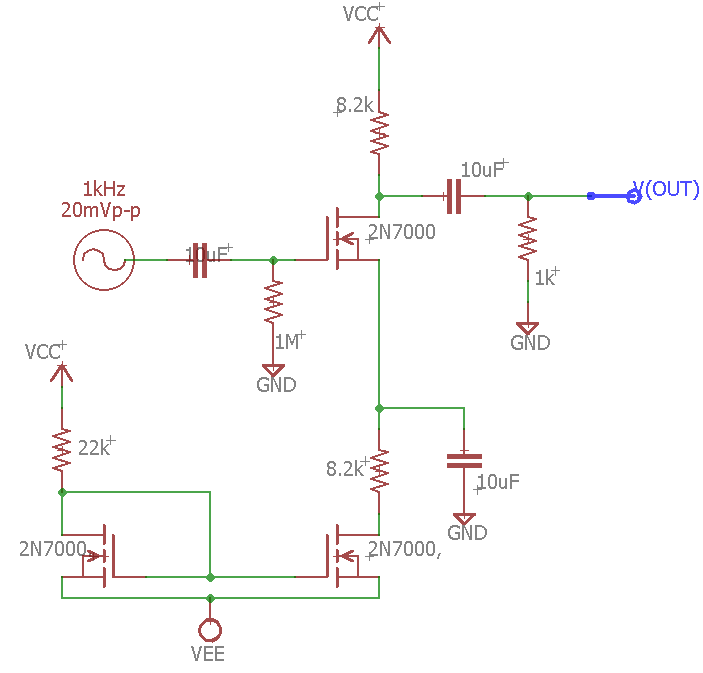
\includegraphics[width=0.7\linewidth]{ExperimentalImplementation/NMOS_exp}
	\caption{NMOS final circuit schematic}
	\label{fig:nmosexp}
\end{figure}
Some of the resistor values had to be changed in order to meet specifications. The capacitors had to be increased as well due to the poor performance of the equivalent nominal value electrolytics. The implemented capacitors are parallel plate which operate better at higher frequencies. Figure \ref{fig:nmosfreq} demonstrates the experimental frequency response of the NMOS amplifier. 


\begin{figure}[H]
	\centering
	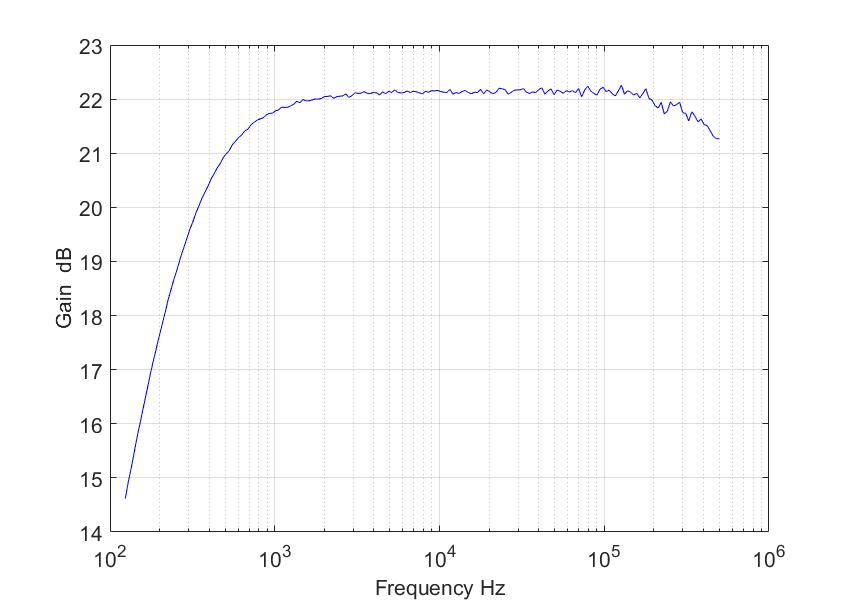
\includegraphics[width=0.7\linewidth]{ExperimentalImplementation/nmosamp.jpg}
	\caption{NMOS experimental frequency response}
	\label{fig:nmosfreq}
\end{figure}

The gain was just on the high end of the specification at 22 dB. The lower cutoff frequency is less than 1 kHz. The upper cutoff also meets spec by being greater than 200 kHz. The FFT of the circuit can by seen in Figure \ref{fig:nmosexpfft}.

\begin{figure}[H]
	\centering
	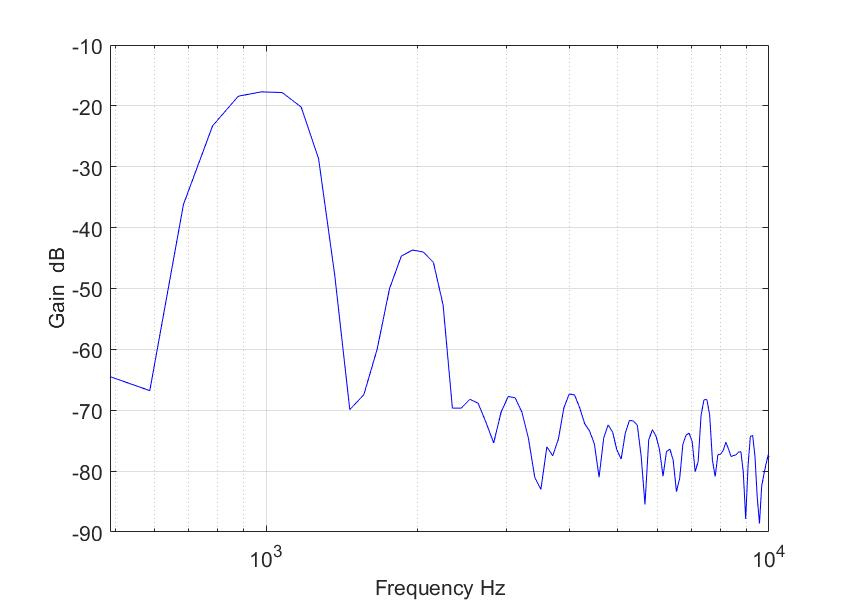
\includegraphics[width=0.7\linewidth]{ExperimentalImplementation/nmos_fft.jpg}
	\caption{NMOS experimental FFT}
	\label{fig:nmosexpfft}
\end{figure}

The second harmonic distortion was slightly too high at 5\%. This can be altered by the negative bias voltage, for the purpose of this lab, 5\% was deemed acceptable. Table \ref{tab:nmosexp} shows the summary of the experimental NMOS circuit.


\begin{table}[H]
	\centering
	\caption{NMOS experimental values}
	\label{tab:nmosexp}
	\begin{tabular}{cc}
		$Q_1, Q_2, Q_3$ & 2N7000        \\ \hline
		$R_ref$         & 22 k$\Omega$ \\ \hline
		$R_g$           & 1 M$\Omega$  \\ \hline
		$R_d$           & 8.2 k$\Omega$   \\ \hline
		$R_s$           & 8.2 k$\Omega$  \\ \hline
		$R_L$           & 1k$\Omega$    \\ \hline
		$C_B$, $C_C$, $C_E$ & 10 $\mu$F         \\ \hline   
		Gain            & 21 dB   \\   \hline
		Lower cutoff    & 600 Hz \\ \hline
		Upper cutoff    & 10  MHz \\ \hline
	\end{tabular}
\end{table}

After minor alterations the circuit operated correctly.



\subsection{BJT amplifier}

The BJT required only a slight change of capacitor values, due to availability. Figure \ref{fig:bjtexp} shows the final circuit for the BJT amplifier circuit.

\begin{figure}[H]
	\centering
	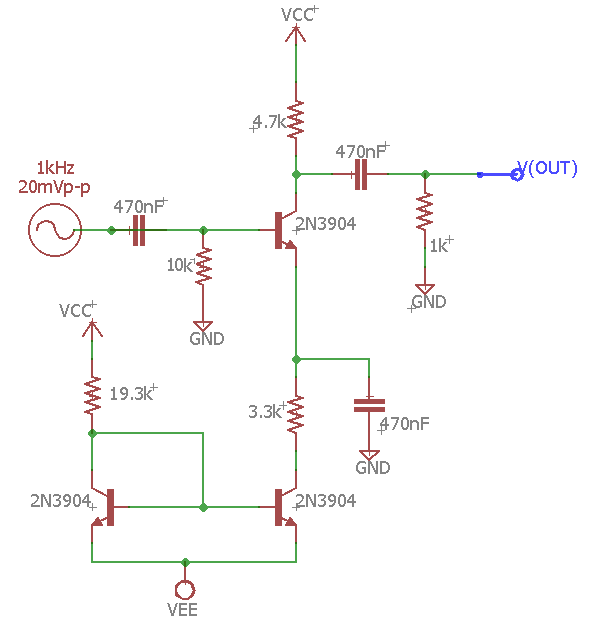
\includegraphics[width=0.7\linewidth]{ExperimentalImplementation/BJT_Exp}
	\caption{BJT final schematic}
	\label{fig:bjtexp}
\end{figure}

The BJT was built using the provided components. The experimental frequency response of the circuit is shown in Figure \ref{fig:bjtexpfreq}.



\begin{figure}[H]
	\centering
	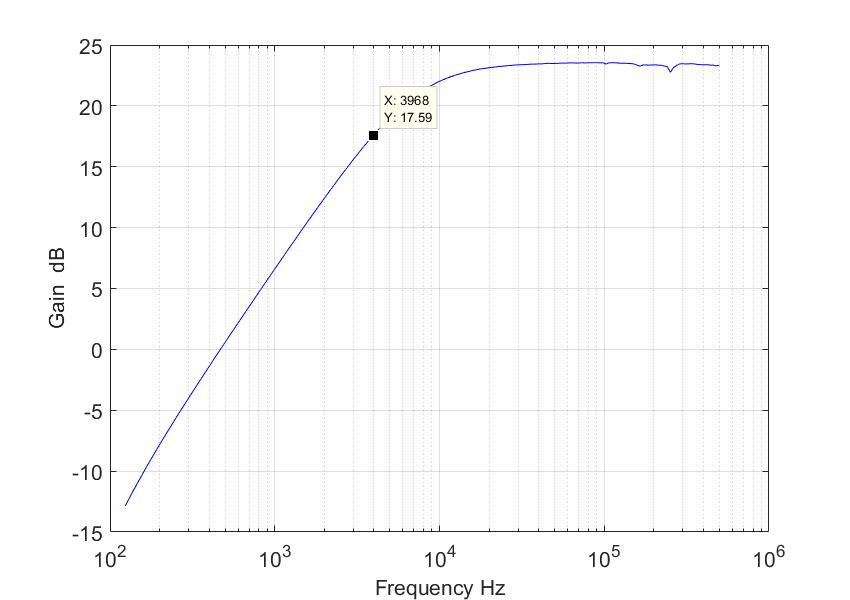
\includegraphics[width=0.7\linewidth]{ExperimentalImplementation/bjt_outputexp.jpg}
	\caption{BJT experimental frequency response}
	\label{fig:bjtexpfreq}
\end{figure}
The gain was a little less than the simulated, at 24 dB, but the lower cutoff was quite higher at 6 kHz, far higher than the specified 1 kHz. The upper cutoff can not be measured exactly due to the limitations of the Digilent Discovery board's network analyzer. The measured values are only accurate up to 500 kHz. The measured FFT of the BJT can be seen in Figure \ref{fig:bjtexpfft}.

\begin{figure}[H]
	\centering
	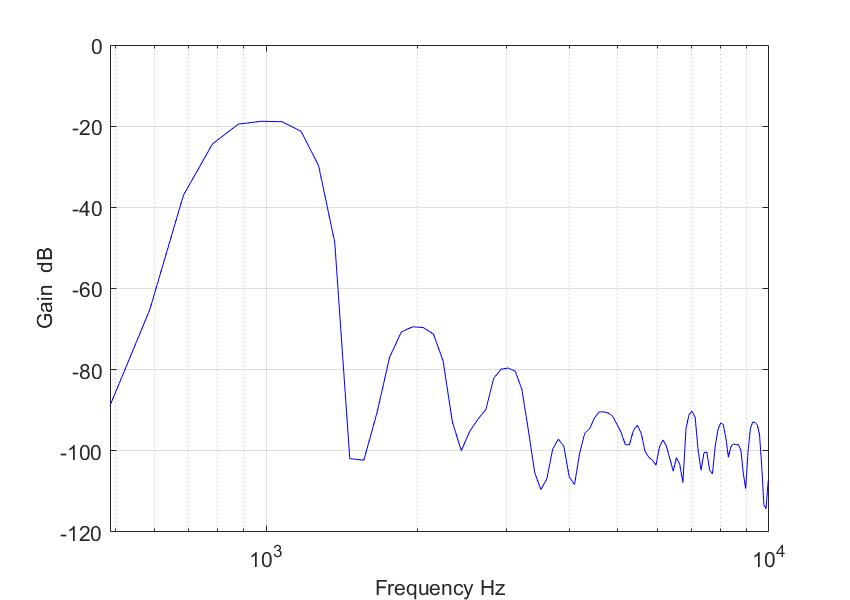
\includegraphics[width=0.7\linewidth]{ExperimentalImplementation/bjt_fft.jpg}
	\caption{BJT experimental FFT}
	\label{fig:bjtexpfft}
\end{figure}

The second harmonc distortion was significantly less than the NMOS while still being in spec, at roughly 1\%. Table \ref{tab:bjtexp} shows the summary of the BJT performance.




\begin{table}[H]
	\centering
	\caption{BJT experimental values}
	\label{tab:bjtexp}
	\begin{tabular}{cc}
		$Q_1, Q_2, Q_3$ & 2N3904        \\ \hline
		$R_ref$         & 19.3k$\Omega$ \\ \hline
		$R_C$           & 4.7k$\Omega$  \\ \hline
		$R_B$           & 10k$\Omega$   \\ \hline 
		$R_E$           & 3.3k$\Omega$  \\ \hline 
		$R_L$           & 1k$\Omega$    \\ \hline
		$C_B$, $C_C$, $C_E$ & 470nF     \\ \hline
		Gain           & 25 dB          \\ \hline
		Lower cutoff   & 6 kHz          \\ \hline
		Upper cutoff   &  >500 kHz      \\ \hline
	\end{tabular}
\end{table}

Overall, the BJT operated as expected, discussion and comparison of the two circuits can be found in Discussion.


%\subsection{Ring oscillator}
%\subfile{ExperimentalImplementation/ringosc.tex}



\end{document}